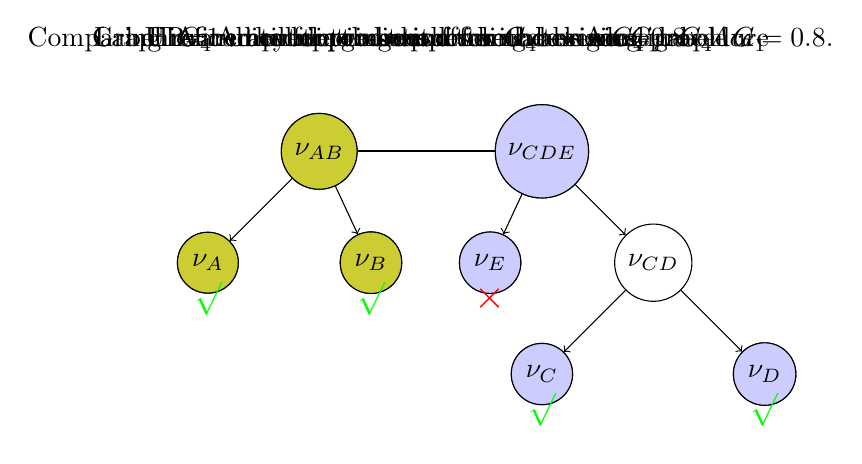
\begin{tikzpicture}
\tikzset{classA/.style={circle, draw=black, fill=blue!20!yellow}, node distance=2cm}
\tikzset{classB/.style={circle, draw=black, fill=blue!20}, node distance=2}
\tikzset{classX/.style={circle, draw=black, fill=red!20}, node distance=2cm}
\tikzset{class0/.style={circle, draw=black}, node distance=2cm}
\tikzset{graphEdge/.style={thick, draw=black}}
\tikzset{treeEdge/.style={draw=black, ->}}


\uncover<1>{\node[draw=none, inner sep=0pt] (ABCDE) {Graph $G_4$ -- the fourth step of the coarsening procedure};}
\node[class0, below left of=ABCDE] (AB) {$\nu_{AB}$};
\node[class0, below right of=ABCDE] (CDE) {$\nu_{CDE}$};
\draw[graphEdge] (AB)--(CDE);
\uncover<2>{
\node[draw=none, inner sep=0pt] (ABCDE) {A model prediction for nodes in $G_4$};
}
\uncover<2->{
\node[classA, below left of=ABCDE] {$\nu_{AB}$};
\node[classB, below right of=ABCDE] {$\nu_{CDE}$};
}
\uncover<3>{
\node[draw=none, inner sep=0pt] (ABCDE) {Hierarchical tree corresponding to nodes in $G_4$};}
\uncover<3->{
\node[class0, below left of=AB] (A) {$\nu_A$};
\node[class0, below right of=AB, xshift=-5ex] (B) {$\nu_{B}$};
\node[class0, below left of=CDE, xshift=5ex] (E) {$\nu_E$};
\node[class0, below right of=CDE] (CD) {$\nu_{CD}$};
\node[class0, below left of=CD] (C) {$\nu_{C}$};
\node[class0, below right of=CD] (D) {$\nu_{D}$};
\draw[treeEdge] (AB)--(A);
\draw[treeEdge] (AB)--(B);
\draw[treeEdge] (CDE)--(E);
\draw[treeEdge] (CDE)--(CD);
\draw[treeEdge] (CD)--(C);
\draw[treeEdge] (CD)--(D);
}

\uncover<4>{
\node[draw=none, inner sep=0pt] (ABCDE) {Label refinement into nodes from the original graph $G_1$};
}
\uncover<4->{
\node[classA, below left of=AB] {$\nu_A$};
\node[classA, below right of=AB, xshift=-5ex] {$\nu_{B}$};
\node[classB, below left of=CDE, xshift=5ex] {$\nu_E$};
\node[classB, below left of=CD] {$\nu_{C}$};
\node[classB, below right of=CD] {$\nu_{D}$};
}

\uncover<5>{
\node[draw=none, inner sep=0pt] (ABCDE) {Comparing refined prediction with true labels on $G_1 \to$ $Acc=0.8$.};
}
\uncover<5->{
 \node[below of=A, node distance=3ex, color=green] {{\large{$\bm{\surd}$}}};
 \node[below of=B, node distance=3ex, color=green] {{\large{$\bm{\surd}$}}}; 
 \node[below of=C, node distance=3ex, color=green] {{\large{$\bm{\surd}$}}}; 
  \node[below of=D, node distance=3ex, color=green] {{\large{$\bm{\surd}$}}}; 
  \node[below of=E, node distance=3ex, color=red] {{\Large{$\bm{\times}$}}};  
}
\uncover<6>{
\node[draw=none, inner sep=0pt]  {\alert{Accuracy upper-bound} for $G_4$ $\to$ Acc=0.8};
}
\uncover<7>{
\node[draw=none, inner sep=0pt]  {UB=1 until merging nodes with \alert{the same label}
};}

\end{tikzpicture}
